\chapter{Humanoid robot: LLR model}\label{app:LeoWalking}

\section{LLR estimate of all state-variables}

In section \ref{sec:LLR-robot leo} we have showed how \ac{LLR} was used to estimate the walking motion of a humanoid robot. For clarity we showed only three representative state-variables. The \ac{LLR} estimates of all 18 state-variables are shown in \figref{fig:LLR-LeoFullMemStep_all_a} and \ref {fig:LLR-LeoFullMemStep_all_b} of this Appendix. The model was estimated using a large estimation dataset ($N=8000$) as memory. The state-transitions were estimated using $K=40$ nearest neighbors. As before, we only show the estimate of one stride (two steps). It is clear that the \ac{LLR} model is able to model all 18 state-variables very accurately. 

\begin{figure}[htbp]
\centering
\subfigure{
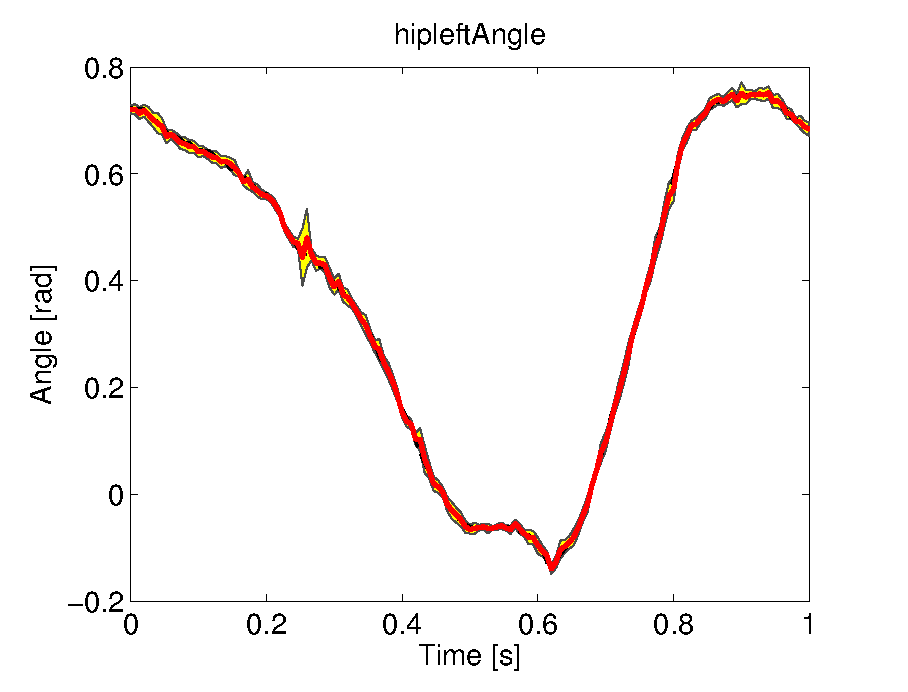
\includegraphics[width=.3\textwidth]{Figures/LLR-LeoFullMemStep_1}
\label{fig:LLR-LeoFullMemStep_1}
}
\subfigure{
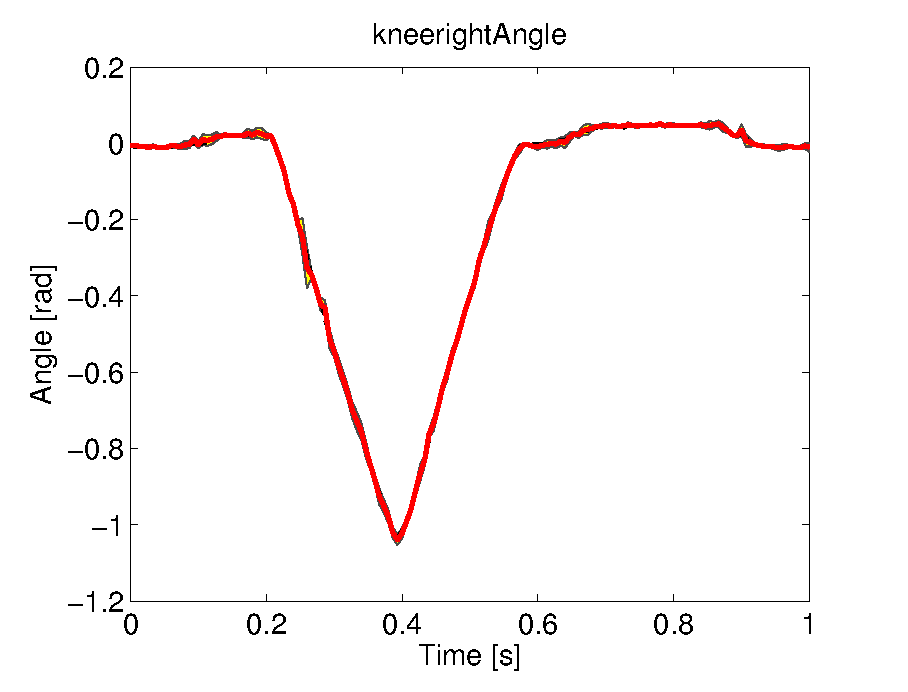
\includegraphics[width=.3\textwidth]{Figures/LLR-LeoFullMemStep_7}
\label{fig:LLR-LeoFullMemStep_7}
}
\subfigure{
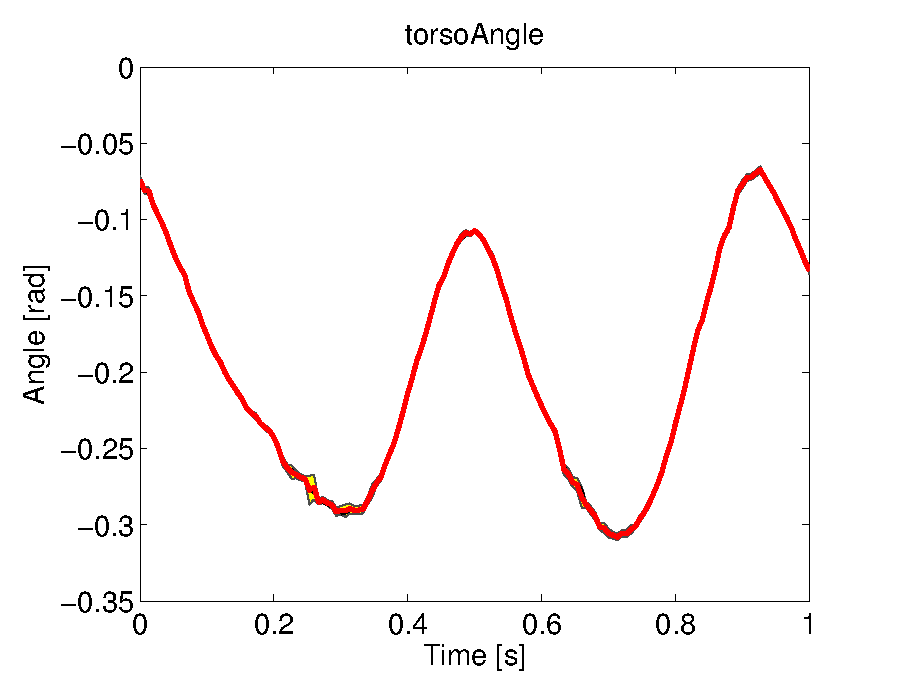
\includegraphics[width=.3\textwidth]{Figures/LLR-LeoFullMemStep_13}
\label{fig:LLR-LeoFullMemStep_13}
} \\
\subfigure{
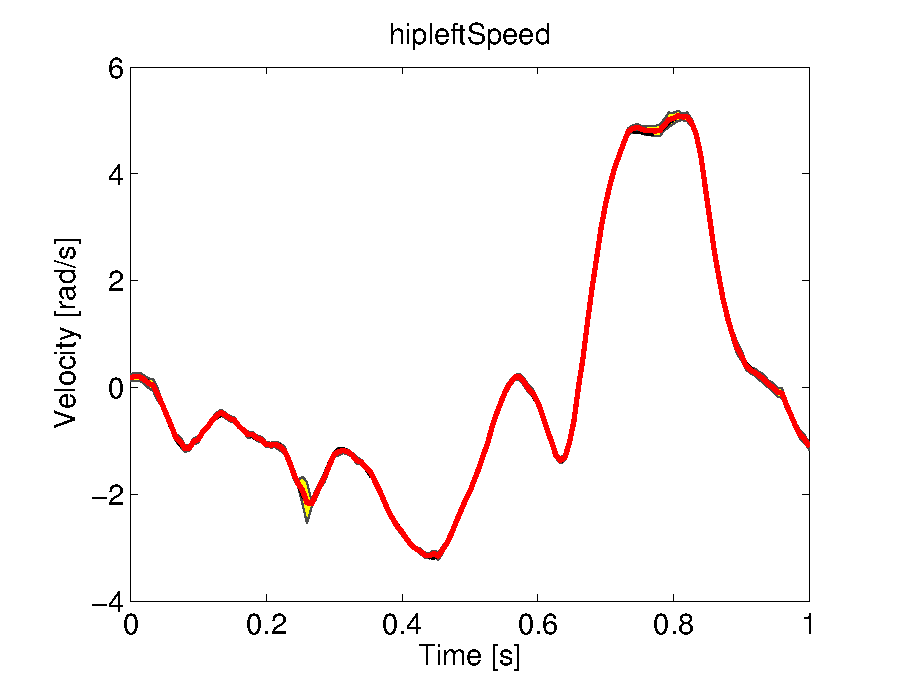
\includegraphics[width=.3\textwidth]{Figures/LLR-LeoFullMemStep_2}
\label{fig:LLR-LeoFullMemStep_2}
}
\subfigure{
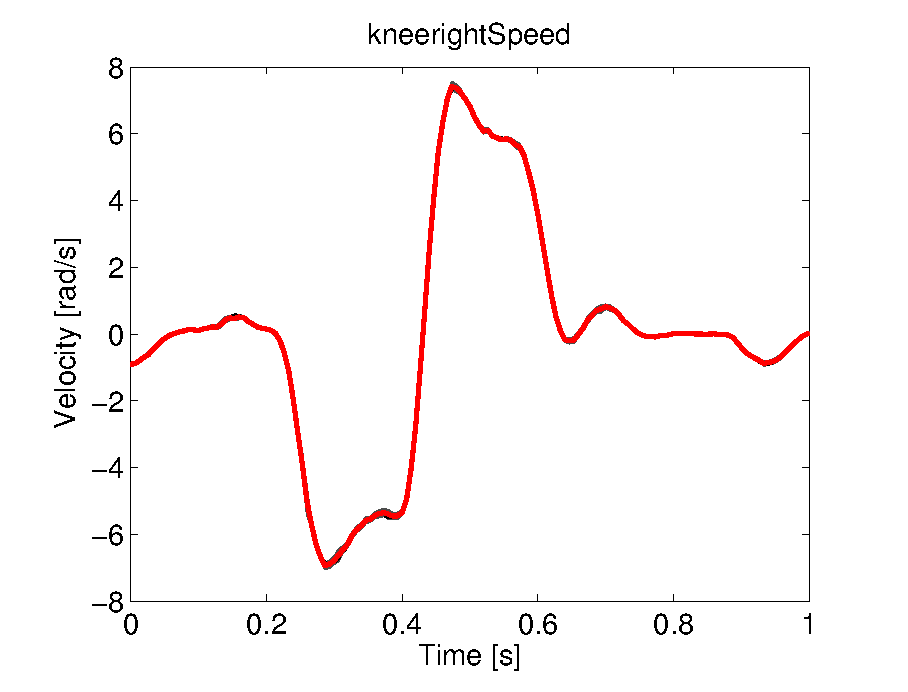
\includegraphics[width=.3\textwidth]{Figures/LLR-LeoFullMemStep_8}
\label{fig:LLR-LeoFullMemStep_8}
}
\subfigure{
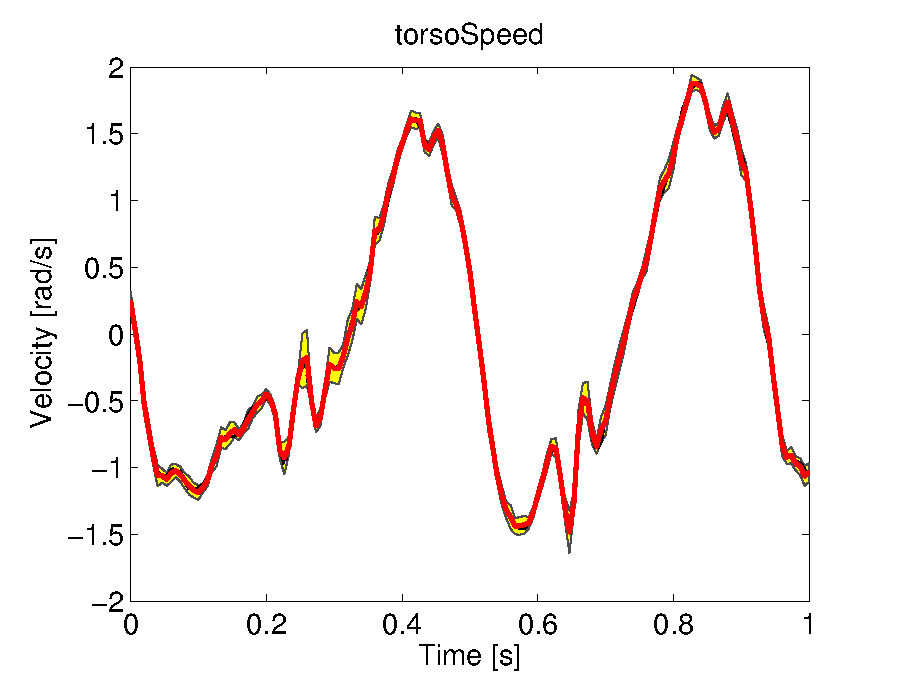
\includegraphics[width=.3\textwidth]{Figures/LLR-LeoFullMemStep_14}
\label{fig:LLR-LeoFullMemStep_14}
} \\
\subfigure{
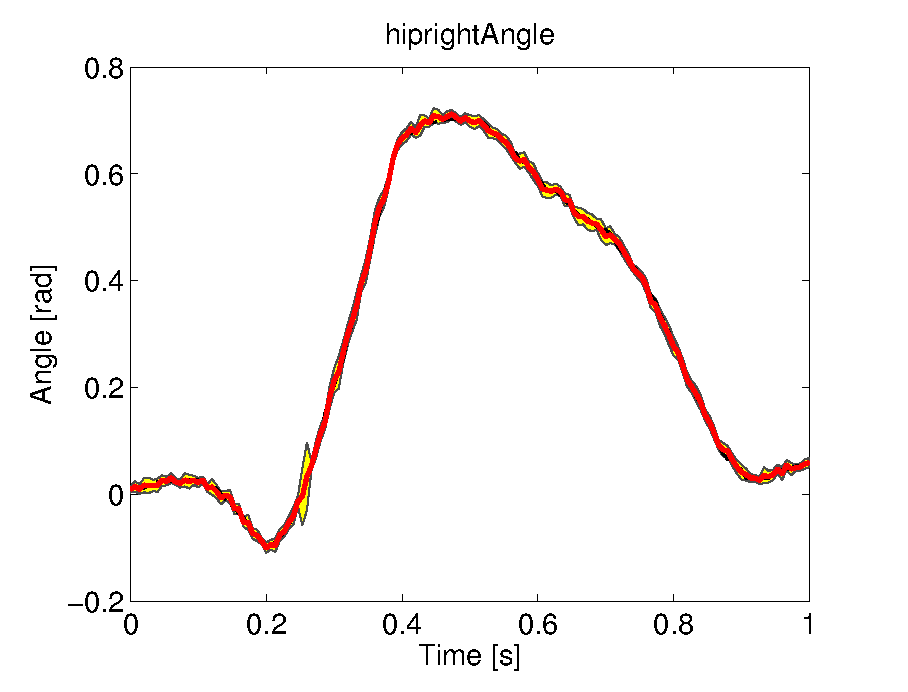
\includegraphics[width=.3\textwidth]{Figures/LLR-LeoFullMemStep_3}
\label{fig:LLR-LeoFullMemStep_3}
}
\subfigure{
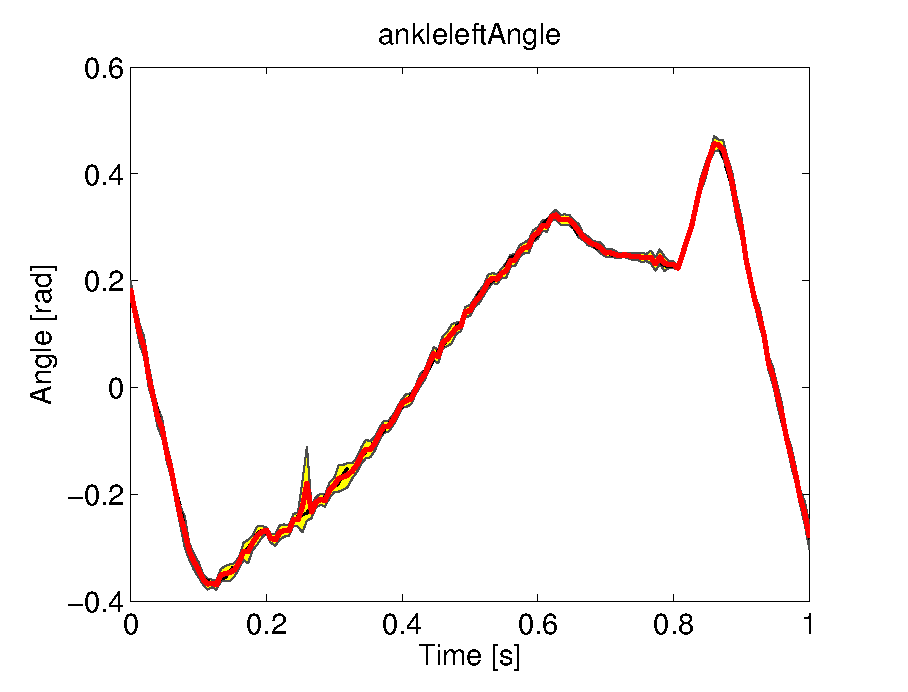
\includegraphics[width=.3\textwidth]{Figures/LLR-LeoFullMemStep_9}
\label{fig:LLR-LeoFullMemStep_9}
}
\subfigure{
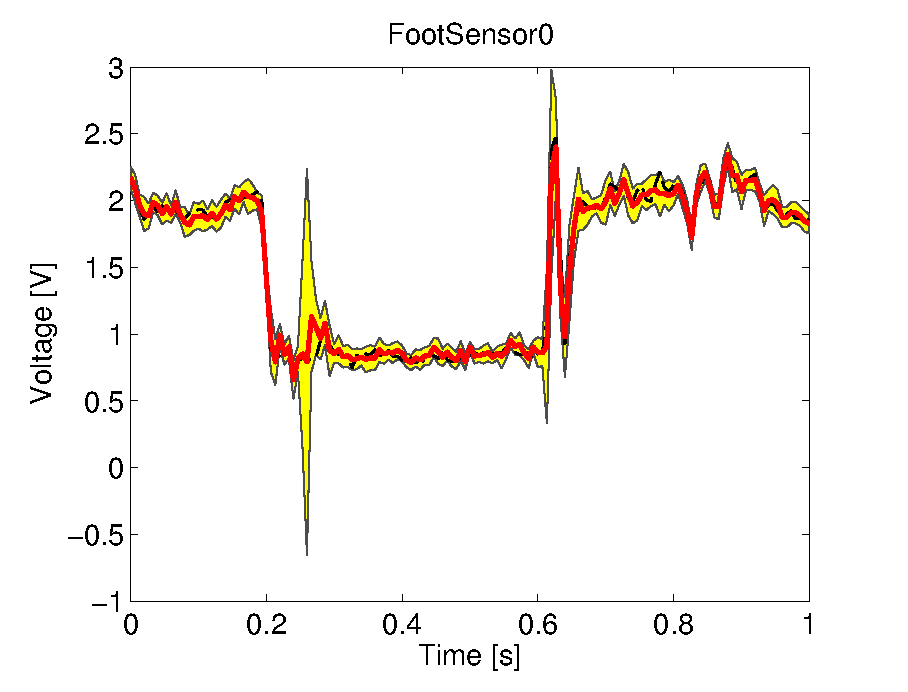
\includegraphics[width=.3\textwidth]{Figures/LLR-LeoFullMemStep_15}
\label{fig:LLR-LeoFullMemStep_15}
} 
\caption[\ac{LLR} estimate of Leo walking, state-variables 1-9]{\ac{LLR} estimate ($K=40$) of the walking motion of robot Leo using a memory consisting of 8000 samples. The figures show 9 different state-variables. The figures show the \ac{LLR} estimate (solid red line), the measured output (dashed black line) and the prediction interval (shaded area).}
\label{fig:LLR-LeoFullMemStep_all_a}
\end{figure}


\begin{figure}[htbp]
\centering
\subfigure{
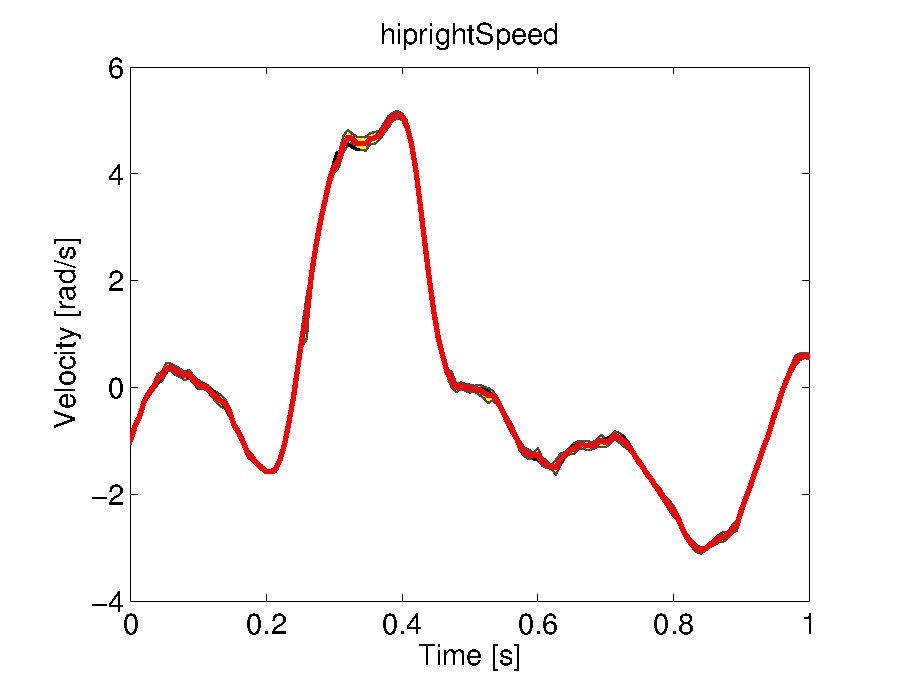
\includegraphics[width=.3\textwidth]{Figures/LLR-LeoFullMemStep_4}
\label{fig:LLR-LeoFullMemStep_4}
}
\subfigure{
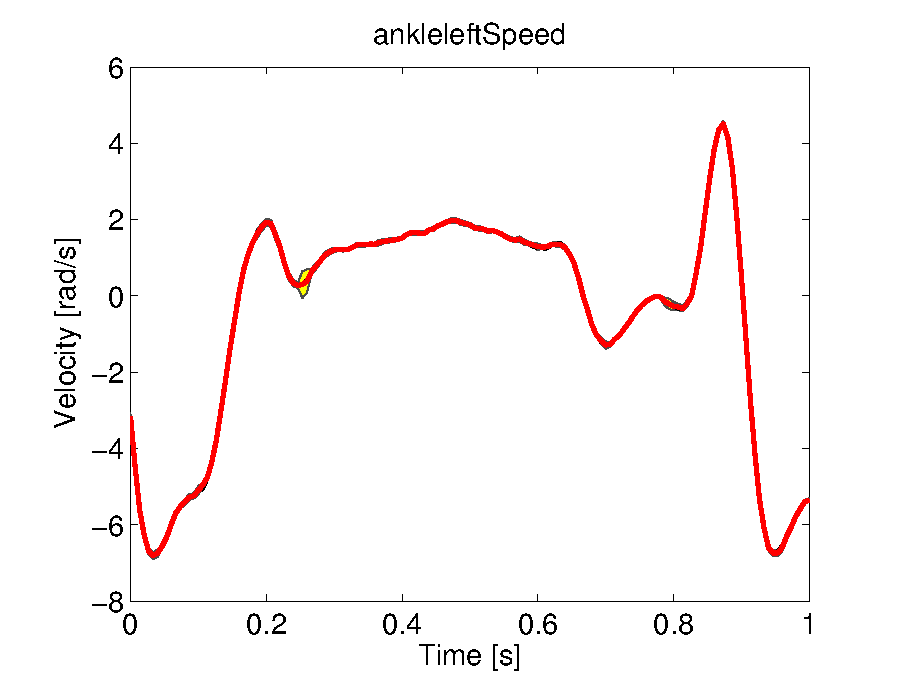
\includegraphics[width=.3\textwidth]{Figures/LLR-LeoFullMemStep_10}
\label{fig:LLR-LeoFullMemStep_10}
}
\subfigure{
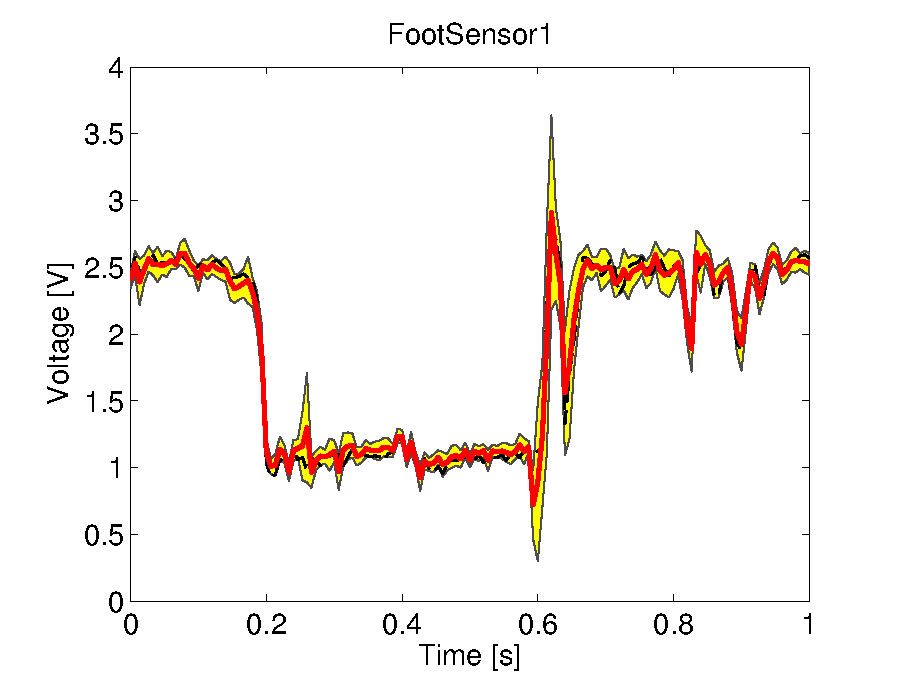
\includegraphics[width=.3\textwidth]{Figures/LLR-LeoFullMemStep_16}
\label{fig:LLR-LeoFullMemStep_16}
} \\
\subfigure{
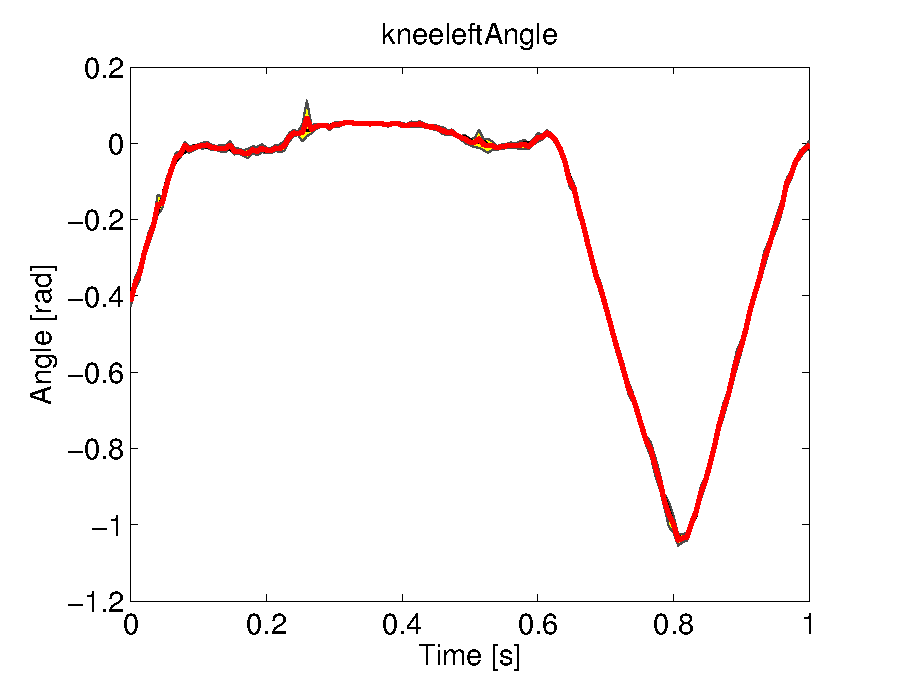
\includegraphics[width=.3\textwidth]{Figures/LLR-LeoFullMemStep_5}
\label{fig:LLR-LeoFullMemStep_5}
}
\subfigure{
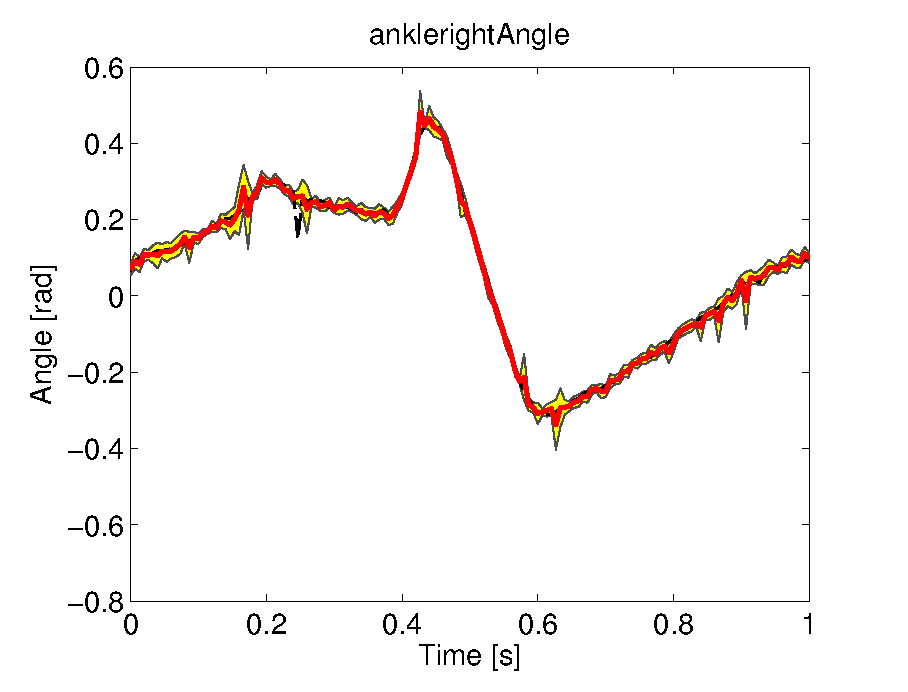
\includegraphics[width=.3\textwidth]{Figures/LLR-LeoFullMemStep_11}
\label{fig:LLR-LeoFullMemStep_11}
}
\subfigure{
\includegraphics[width=.3\textwidth]{Figures/LLR-LeoFullMemStep_17}
\label{fig:LLR-LeoFullMemStep_17}
} \\
\subfigure{
\includegraphics[width=.3\textwidth]{Figures/LLR-LeoFullMemStep_6}
\label{fig:LLR-LeoFullMemStep_6}
}
\subfigure{
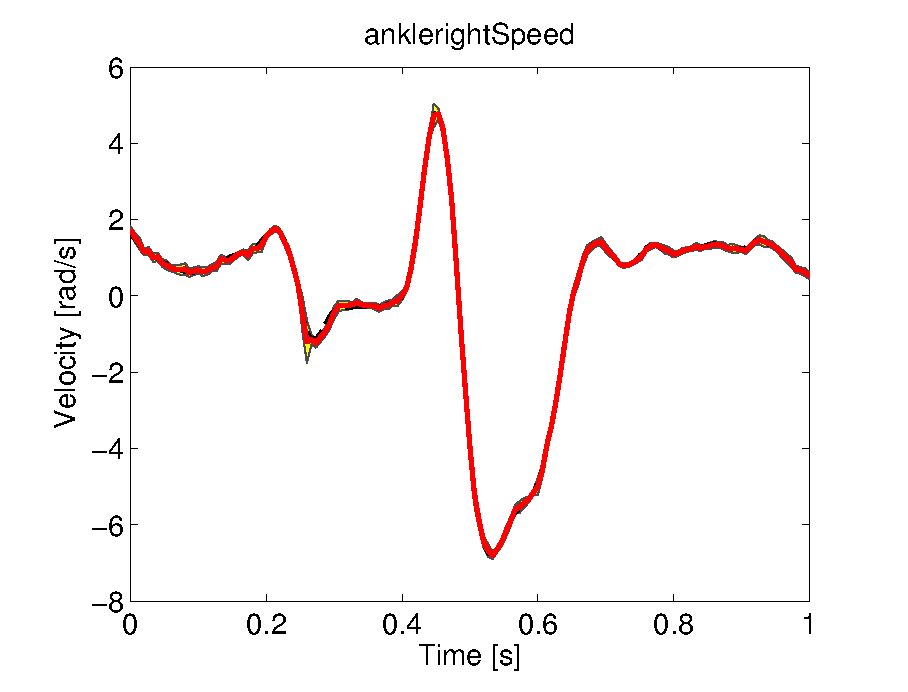
\includegraphics[width=.3\textwidth]{Figures/LLR-LeoFullMemStep_12}
\label{fig:LLR-LeoFullMemStep_12}
}
\subfigure{
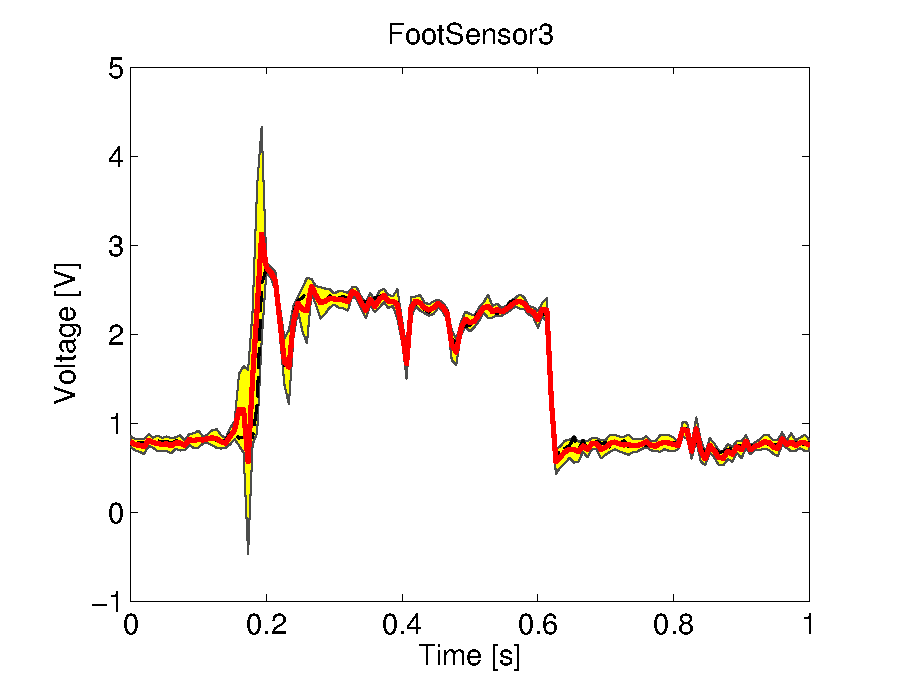
\includegraphics[width=.3\textwidth]{Figures/LLR-LeoFullMemStep_18}
\label{fig:LLR-LeoFullMemStep_18}
} 
\caption[\ac{LLR} estimate of Leo walking, state-variables 10-18]{\ac{LLR} estimate ($K=40$) of the walking motion of robot Leo using a memory consisting of 8000 samples. The figures show 9 different state-variables. The figures show the \ac{LLR} estimate (solid red line), the measured output (dashed black line) and the prediction interval (shaded area).}
\label{fig:LLR-LeoFullMemStep_all_b}
\end{figure}